\chapter{State of the Art}\label{chapter:state-of-the-art}
This chapter presents an overview of state of the art approaches to object recognition, while focusing on two families of architectures, which are motivated quite differently. Object recognition techniques based on convolutional neural networks (\emph{CNN}s) currently dominate the field, achieving state of the art performance on many datasets \cite{Diba2017WeaklySC,7506134}. CNNs however, are only loosely based on biological neurons. Spiking neural networks (\emph{SNN}s) on the other hand, try to mimic the physical properties of neurons more closely and therefore constitute biologically more plausible models \cite{Schofield20180027}. Generally speaking, CNNs may be regarded as a more engineering-based approach (or top-down), while SNNs are motivated by results from neuroscience and biology (bottom-up approach).
\section{Deep Learning for Object Recognition}
Recent years have seen a surge of interest in deep learning methods, especially in the field of computer vision. While the theory behind many deep learning methods has been around for many years, their recent success is mainly due to the availability of large labelled data sets and highly parallel computing powered by GPUs. One of the specific tasks, deep learning based methods excel at, is object recognition: the identification of objects in images or videos (cf. figure \ref{fig:cifar10}). The significantly better performance of deep neural networks over traditional machine learning methods can be explained by: (i) their hierarchical topology of parameterized non-linear processing units is a fundamentally better probabilistic model and prior for real world data leading to better generalization and (ii) they automatically find good features to extract based on the training data.
\begin{figure}[htpb]
    \centering
\begin{tikzpicture}
  \node[anchor=south west,inner sep=0] at (0,0) {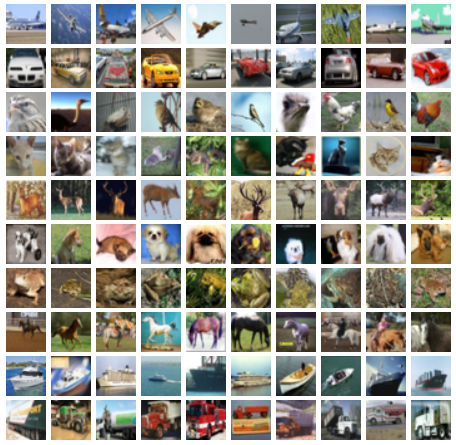
\includegraphics{figures/cifar10.png}};
  \node[anchor=west] at (-2.5,8.9) {Airplane};
  \node[anchor=west] at (-2.5,7.95) {Automobile};
  \node[anchor=west] at (-2.5,7.05) {Bird};
  \node[anchor=west] at (-2.5,6.1) {Cat};
  \node[anchor=west] at (-2.5,5.2) {Deer};
  \node[anchor=west] at (-2.5,4.25) {Dog};
  \node[anchor=west] at (-2.5,3.35) {Frog};
  \node[anchor=west] at (-2.5,2.45) {Horse};
  \node[anchor=west] at (-2.5,1.5) {Ship};
  \node[anchor=west] at (-2.5,.55) {Truck};
\end{tikzpicture}
\caption[CIFAR-10 classes and sample images]{Sample images from the CIFAR-10 \cite{cifar10} dataset and their corresponding classes. CIFAR-10 consists of 6000 images at 32 by 32 pixels for each of the 10 classes. Datasets such as this are often used as a benchmark to evaluate the performance of novel deep learning architectures for image recognition.}\label{fig:cifar10}
\end{figure}
The potential applications for a robust image classification system are myriad and range from automated driving and image-based diagnosis to robot vision and many more. As deep learning is currently the best candidate for such a system, it is well worth exploring.
\subsection{Convolutional Neural Networks}
CNN architectures are generally distinguished by their use of specific types of neuron-layers, namely, convolutional, pooling and fully connected layers. While wildly different network topologies may be found in literature, characterized by their use of skip connections, number of layers, number of paths etc., CNNs can always be reduced to these three basic layer types.
\subsubsection{Fully Connected Layer}
Each neuron in a fully connected layer is connected to all the activations in the previous layer. The activation of a single neuron as the basic non-linear computational unit is calculated by applying a nonlinearity to the weighted sum of its inputs plus a bias.
\begin{align}
    h = g\qty(\sum_i w_i x_i +b)
\end{align}
With the nonlinear function $g$, the learnable weights $w_i$, the input activations $x_i$ and the learnable bias $b$. In the case of a fully connected layer, the activation can be computed using matrix multiplication. In tensor notation this may be written as:
\begin{align}
    \vb{h_l} = g_l\qty(\vb{W^T_l\vb{h_{l-1}}}+\vb{b_l}).
\end{align}
With $N_l$ denoting the number of neurons in layer $l$, $\vb{W_l}$ is an $N_{l-1}\cp N_l$ dimensional weight matrix, $b_l$ an $N_l$ dimensional vector and $g_l$ the $N_l$ dimensional vectorized activation function of layer $l$
\begin{align}
    g_l(\vb{x}) = \qty(g_l(x_1),...,g_l(x_{N_l}))^T
\end{align}
\subsubsection{Convolutional Layer}
\subsubsection{Pooling Layer}
\subsection{Spiking Neural Networks}
\section{Limits of Deep Learning Approaches}